\section{Training}

% hablar lo que que tenemos y lo que estamos haciendo
% tenemos el la arquitectura definida, con el feature set y sabemos que da un numerito. ahora hay qeu definir con que datos lo entrenamos y qué es el numerito que buscamos (a partir de los datos)

Given a feature set, the network architecture is completely defined, along with how to encode a position into its inputs. This section will describe the two methods to train the networks, each with its own loss function and training dataset.
[mas?]

\subsection{Source dataset}

Data is needed to train the network. The proposal for the thesis was to use the Lichess database \cite{lichessdb}, which provides a CC0 database with all the games ever played on the site, then score the positions using Stockfish. After some initial experiments, the networks were not performing as expected. Upon further reaserch I found out that I was working with datasets too small for this task (order of hundreds of millions). I needed a larger dataset (order of \textbf{dozens of billions}), but it was impractical for me to generate it. Fortunately, I can use the same dataset that Stockfish uses to train their networks \cite{sf_nnue_dataset}, which should work well. Specifically, I went with the dataset used to train the first stage of the main network for Stockfish 16.1, which is 135GB of compressed \texttt{binpack} files. It was built by running Stockfish at 5000 nodes on multiple opening books. Later stages datasets generated by Leela Chess Zero (LC0), which is more expensive to compute but has a higher quality evaluations.

The \texttt{binpack} format is a very efficient format to store samples yet very complex to decode. Fortunately, Stockfish provides a tool to export this data into a text format. I had to modify it to export it in the format I wanted. I changed the \texttt{emitPlainEntry} function in \texttt{nnue\_data\_binpack\_format.h} to the code in Appendix \ref{appendix:emitPlainEntry}. The resulting file was 2.59TB in size and contained \textbf{48.4 billion samples} with the format:

\begin{center}
\begin{tabular}{|cp{0.0005cm}cp{0.0005cm}c|}
\hline
\textbf{FEN\footnotemark} & , & \textbf{Score} & , & \textbf{Best move} \\
\hline
\end{tabular}
\end{center}

\footnotetext{Standard notation to describe positions of a chess game. It is a sequence of ASCII characters.}

The file was too big to be practical and it would wear off my SSD, so I made a tool to compact the data into a similar format. The new format expoits the fact that samples in a row belong to the same game. This means that contiguous FENs are a move from a previous one, so it stores the move instead of the FEN:

\begin{center}
\begin{tabular}{|cp{0.0005cm}cp{0.0005cm}c|}
\hline
\textbf{FEN} & , & \textbf{Score} & , & \textbf{Best move} \\
\hline
\end{tabular}
(
\begin{tabular}{|p{0.0005cm}cp{0.0005cm}cp{0.0005cm}c|}
\hline
, & \textbf{Actual move} & , & \textbf{Score} & , & \textbf{Best move} \\
\hline
\end{tabular}
) *\footnote{Repeated zero or more times.}
\end{center}

As you can see, the new format is compatible with the last one, so only one reader was implemented. After compacting the data, the file went down to a manageable 522GB.

Each training method will generate a new derived dataset based on this samples, to later train the network.

% Lichess is a free online site to play chess, and thankfully it provides a CC0 database \cite{lichessdb} with all the games ever played on the site. It consists of serveral compressed PGN files\footnote{Portable Game Notation: a textual format to store chess games (moves and metadata)} splitted by month since 2013, that add up to $1.71$TB compressed. The whole database contains over 5.5 billion games, that equates to around 200 billion positions. In practice, that many positions are too much to handle so I'll use only a fraction of them and take only one sample per game to increase the diversity of positions.

% The Lichess database also provides a database of puzzles
% hablar de esto en otro lado (results? eval?)

% A single game can have lots of positions, most of which are shared with millions of other games, mostly during the early game. This is a problem of its own: trying to sample positions from a game with a suitable distribution. In this work, I have chosen to only consider positions 20 half-moves into the game.

\subsection{Method 1: Score target}

The main method to train the network will use the latest Stockfish evaluations as target. The objective is to train the network to predict the evaluation of a position as Stockfish would do.

First, we need to generate the training data. It is not known what makes a dataset good, but usually you can use the previous version of an engine to evaluate positions to train the next version. Stockfish uses a combination of datasets generated this way and evaluations from Lc0 that are more expensive to compute but have a higher quality, given the type of engine (it uses MCTS with a deep neural network).

I have chosen to generate the training set using evaluations from Stockfish version 16.1 at depth 10, as recommended by the authors of nnue-pytorch \cite{nnue-pytorch}. For each game, I uniformly sample a position (after 20 half-moves), run Stockfish and store the centipawn evaluation.

\setcounter{secnumdepth}{4}
\subsubsection{CP-space to WDL-space}
% I guess it is to steer the old network to the new one while making 

The evaluations from Stockfish are in centipawns, which is not the exact number the network has to use as target.


decir que no usamos el outcome de la partida para el score

\[
L_\varepsilon(y,f(x,w))=
\max\{0, |y-f(x,w)|-\varepsilon\}
\]


\subsubsection{Loss function}

\[
L_\varepsilon(y,f(x,w))=
\max\{0, |y-f(x,w)|-\varepsilon\}
\]


\subsection{Method 2: PQR triplets}

This is an additional technique I wanted to try, described in \cite{dlchess:2014}. Remember that we are trying to obtain a function $f$ (the model) to give an evaluation of a position. The method is based in the assumption that players make optimal or near-optimal moves most of the time, even if they are amateurs.

\begin{enumerate}
\item For two position in succession $p \rightarrow q$  observed in the game, we will have $f(p) \neq f(q)$.
\item Going from $p$, not to $q$, but to a \textit{random} position $p \rightarrow r$, we must have $f(r) > f(q)$ because the random move is better for the next player and worse for the player that made the move.
\end{enumerate}

With infinite compute, $f$ would be the result of running minimax to the end of the game, since minimax always finds optimal moves.


\subsubsection{Loss function}


\[
L_\varepsilon(y,f(x,w))=
\max\{0, |y-f(x,w)|-\varepsilon\}
\]


\subsection{Setup}

% filtering
% filtrar de ante mano no rinde (pierde compresion)

% multithreading
% decir que en "All" tengo 450 it/s (7.3M pos/sec)

The project is written in two languages: Rust and Python. The Rust part is used to process PGN files, generate training data and provide final training batches for Python to consume. The Python part defines the Pytorch model, runs the training loop, quantizes the model and runs the evaluations.

The training process is separated in two steps:

\begin{enumerate}
\item Generate the training data from the Lichess database (the source dataset), for \textbf{a specific method}.
\item Train the network using the generated training data and \textbf{a specific feature set}.
\end{enumerate}

Doing it this way allows to generate the training data once per method and train the network with different feature sets. Since generating the training data is the most time-consuming part of the process and I was iterating lots of different feature sets, it is ideal to have it separated. I could have an intermediate step, to generate the raw batch data from the method and feature set, but it is a waste in terms of practicallity and disk space. \\

As depicted in Figure \ref{fig:database_to_train_data}, the first step takes PGN files from the Lichess database and a training method (in this case \textcolor{orange}{\textit{eval}}, which stands for Stockfish evaluations) and builds a traning dataset from it. In this case, each sample is a FEN position (in \textcolor{red}{red}) and the centipawn evaluation (in \textcolor{blue}{blue}). \\

\begin{figure}[h]
\centering
\makebox[\textwidth]{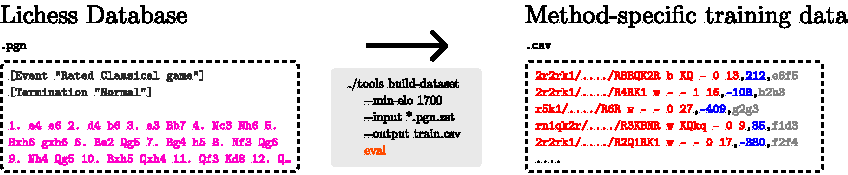
\includegraphics[width=\textwidth]{../assets/training/database_to_train_data.pdf}}
\caption{Diagram of the first step of the training process}
\label{fig:database_to_train_data}
\end{figure}


Once the first step is done, the training can begin. The training process is started by running a Python script (\texttt{scrips/train.py}) and it requires to define the model architecture (number of neurons and hidden layers), general training parameters (learning rate, batch size, epochs, checkpoints, etc) and the feature set to use, which in turn determines the size of the batches. For example, if PQR is used, the size of a sample is 3 times the size of the feature set, and if it is eval, it is the size of the feature set plus 1 for the centipawn evaluation (the target).

The training data obtained in the previous step has to be converted to an actual tensor of floats to be consumed by Pytorch. This is done by a Rust subprocess running the subcommand \texttt{samples-service} that read the training data files and generates training batches for the specified feature set in a shared memory buffer. The Python script copies the data from the buffer at the start of each iteration, allowing Rust to generate the next batch (in the CPU) while Pytorch is training the current one (in the GPU). To coordinate the memory access between the two processes, a single byte is sent using standard I/O.

Given that the input vector is multiple-hot encoded, the data written by the Rust process are not float values. Instead, they are 64-bit integers acting as a bitset. Before passing the vector to the model, it is expanded into floats. This means 64 floats can be packed into a single 64-bit integer, meaning a \textbf{96.875\%} reduction in memory usage (from 256 to 8 bytes). The speedup obtained by this optimization was substantial. The compression can be further improved using sparse tensors, but it is not implemented in this work. \\

[wandb? evaluation?]


